\newpage
\subsubsection{Supermario (by Philipp Haller)}

This part discusses the model used to solve a level of the Supermario game which was presented in section XX. The presented visualisations are generated from the Embedded MontiArc Studio. Therein, a grey component indicates that the component uses additional subcomponents. 

VEREINFACHUNGEN?? WIESO? HIERHIN?

The first entity modelled was the supermario wrapper which is closely related to the outputs and inputs of the simulator. Therefore it receives all necessary values as input with the aim to forward them to the actual controller and its corresponding sub-components. After computation the results of the controller are handed back into the wrapper, which forwards the data to the simulator. Figure XX shows the graphical representation, while listing XX shows the actual EMA interface definition.
\begin{figure}
	\centering
	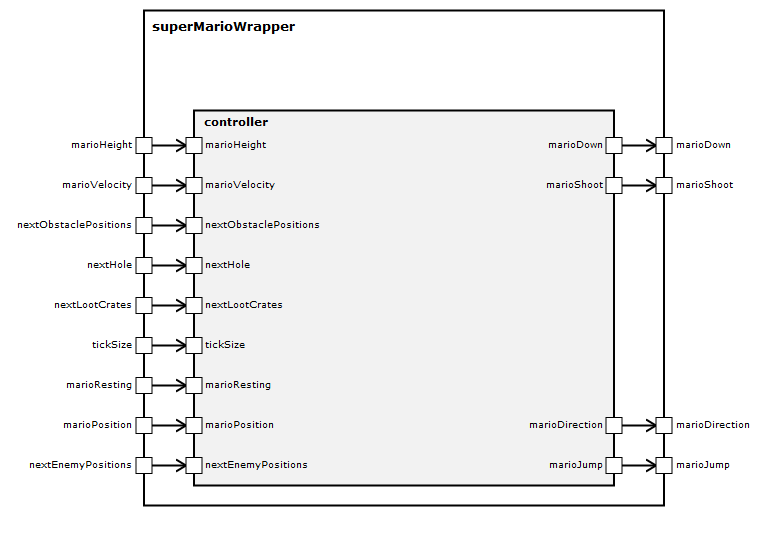
\includegraphics[scale=0.5]{pictures/haller_supermariowrapper.PNG}
	\caption{Visualisation of the Supermario wrapper model}
	\label{fig:marioWrapper}
\end{figure}

\begin{lstlisting}[label=lst:marioWrapperInterface, caption=Interface of the Supermario Wrapper, morekeywords={ports, port, connect, in, out, instance, ->},
frame=single]
    ports   
        in Z^{1,2} marioPosition,
        in Z^{1,2} marioVelocity,
        in Z marioHeight,
        in Z^{5,2} nextEnemyPositions,
        in Z^{5,2} nextObstaclePositions,
        in Z nextHole,
        in Z^{5,2} nextLootCrates,
        in Q tickSize,
        in Z marioResting,
        out Z(-1 : 1 : 1) marioDirection,
        out Z marioJump,
        out Z marioDown,
        out Z marioShoot;
\end{lstlisting}

As inputs the player figure's position, velocity and height were chosen, together with the positions of the next five enemies and obstacles. Furthermore, the position of the next hole in the ground, the position of the next five loot crates, the tick size e.g. time between executions and the information if the player is resting on a tile is given.
The outputs consist of the direction the player shall go in combination with the action instructions jumping, crouching and shooting.

\begin{figure}
	\centering
	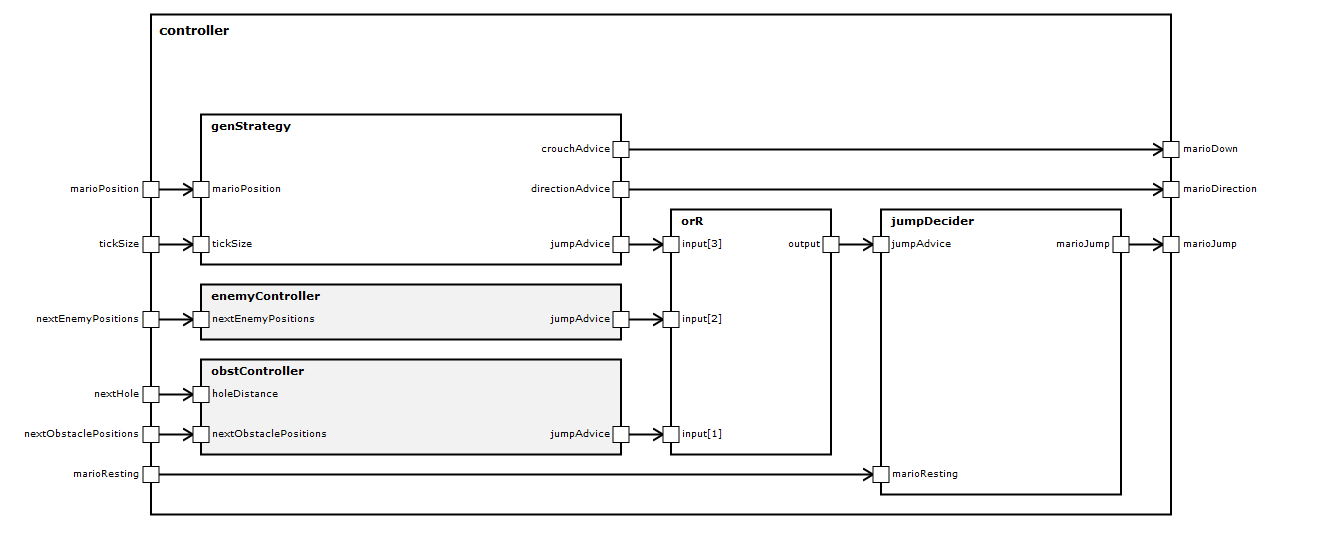
\includegraphics[scale=0.5]{pictures/haller_controller.PNG}
	\caption{Visualisation of the Supermario controller model}
	\label{fig:marioController}
\end{figure}

DONT FORGET TO GIVE DEFINITIONS!
The controller used consists of five parts and is depicted in figure XX. There are sub-controllers tasked to cope with the evaluation of enemies and obstacles respectively, named enemyController and obstController. They return an advice to indicate if the player should jump or not. The genStrategy is an atomic component which is currently used to provide a general strategy like moving in another direction, jumping or crouching if the player is stuck. 

The action advices of the controllers and the strategy are combined via a logical or-relation, as indicated by the "orR" block. Additionally, the jumpDecider filters the output of the combined value and forwards it, if the player can jump in that timeframe. This is necessary to prohibit side-effects like the player only jumping once because the jump key remains pressed constantly and the simulator only accepts distinct jump activations.

\begin{figure}
	\centering
	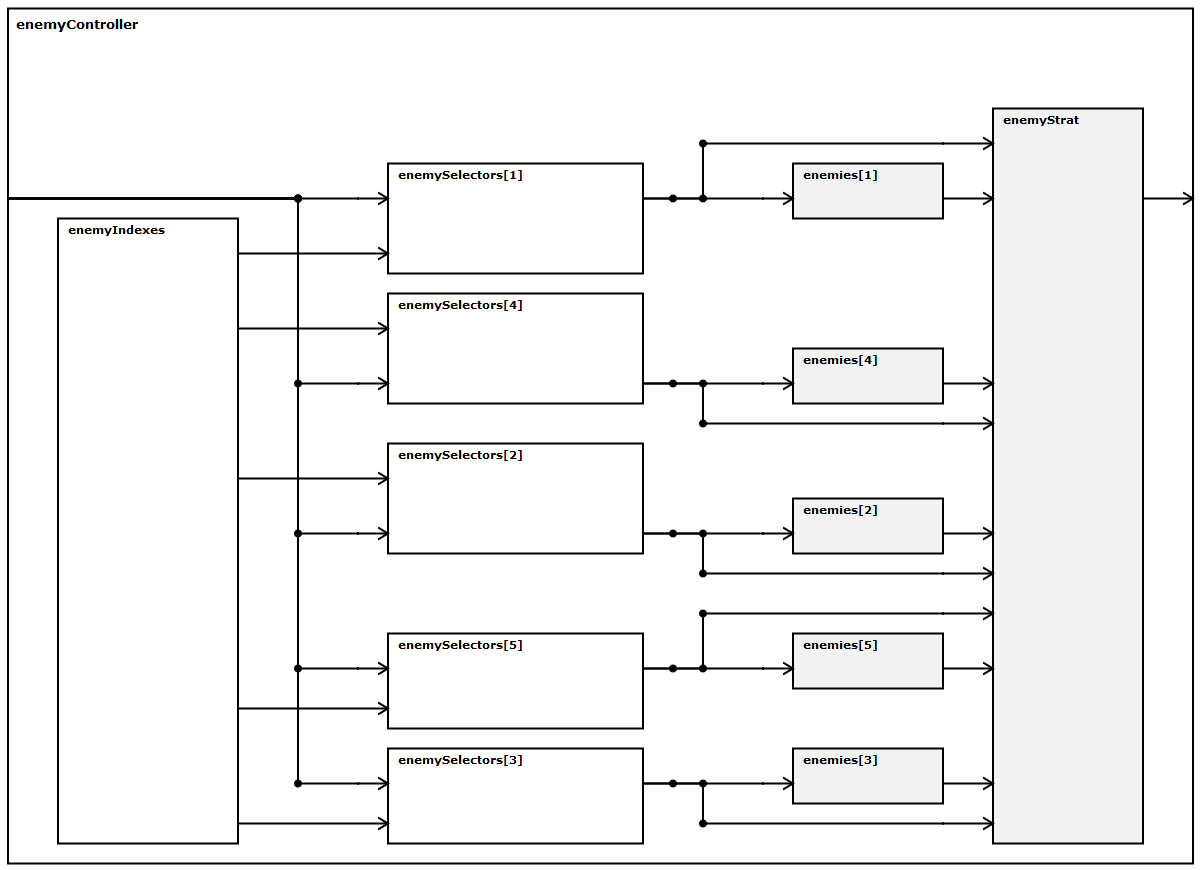
\includegraphics[scale=0.4]{pictures/haller_enemycontroller.PNG}
	\caption{Visualisation of the Supermario enemy controller model}
	\label{fig:marioEnemyController}
\end{figure}

The enemy controller handles the enemy position evaluation and assesses if an action has to be initiated. As the input data from the simulator is a array with five positions, it contains a enemy selector component which returns the corresponding x and y values from a given index. For purposes of overview and readability of the EMA code a component "enemyIndexes" was used to feed these indexes into the selectors.

TBD

\begin{figure}
	\centering
	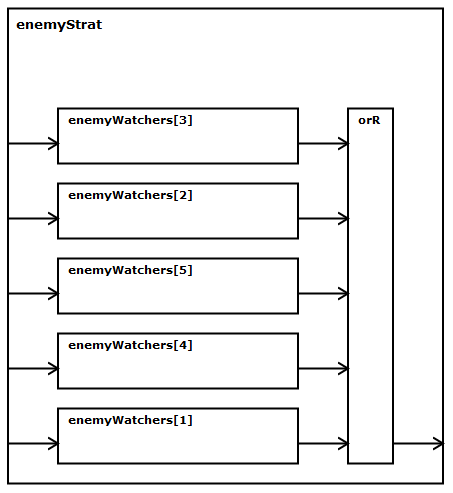
\includegraphics[scale=0.4]{pictures/haller_enemystrategy.PNG}
	\caption{Visualisation of the Supermario enemy strategy model}
	\label{fig:marioEnemyStrategy}
\end{figure}

The enemy strategy uses the distances and velocities from the enemy components to watch them for their distance to the player and wether they can get dangerous. If an enemy comes too close and is on the player's pane, a jump advice is given. The jump advices are again combined via a logical or-relation and returned.


The obstacle controller is modelled very similar to the enemy controller, extracting positions from the raw input array and feeding them into a obstacle strategy. The main difference to the enemy controller is the presence of another input. This additional input is the distance to the next disruption in the ground pane of the level. It is forwarded into the obstacle strategy where a watcher component checks the player's proximity to the hole and emits a jump advice. The advice is then used....

TBD



During modelling of Supermario a distinction between models named with "controller" and "strategy was made.
In scope of the Supermario model the name "controller" was used to describe a model which 

"Watcher"

"Selector"

"Strategy"

"Controller"

"Decider??"





\begin{figure}
	\centering
	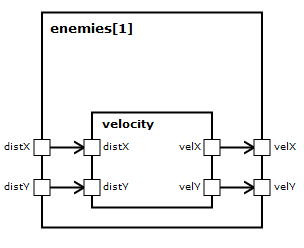
\includegraphics[scale=0.5]{pictures/haller_enemy.PNG}
	\caption{Visualisation of the Supermario enemy model}
	\label{fig:marioEnemy}
\end{figure}




\emph{Execution}

The presented models are executed in